\documentclass[UTF8]{ctexart}
\usepackage{amsmath,amssymb}
\usepackage{mathrsfs}
\usepackage{graphicx}
\usepackage{subfigure}
\usepackage{geometry}
\title{\heiti 引力波作业报告}
\author{\kaishu 刘苏明}
\date{\today}
\geometry{a4paper, left=3.18cm, right = 3.18cm, bottom = 2.54cm, top = 2.54cm}
\begin{document}
\maketitle
\section{数据分析}
从网站[https://www.gw-openscience.org/events/GW150914/]可以获取Living和Hanford的引力波探测数据。
\begin{figure}[!htbp]
	\centering
	\subfigure[未修正的引力波波形]{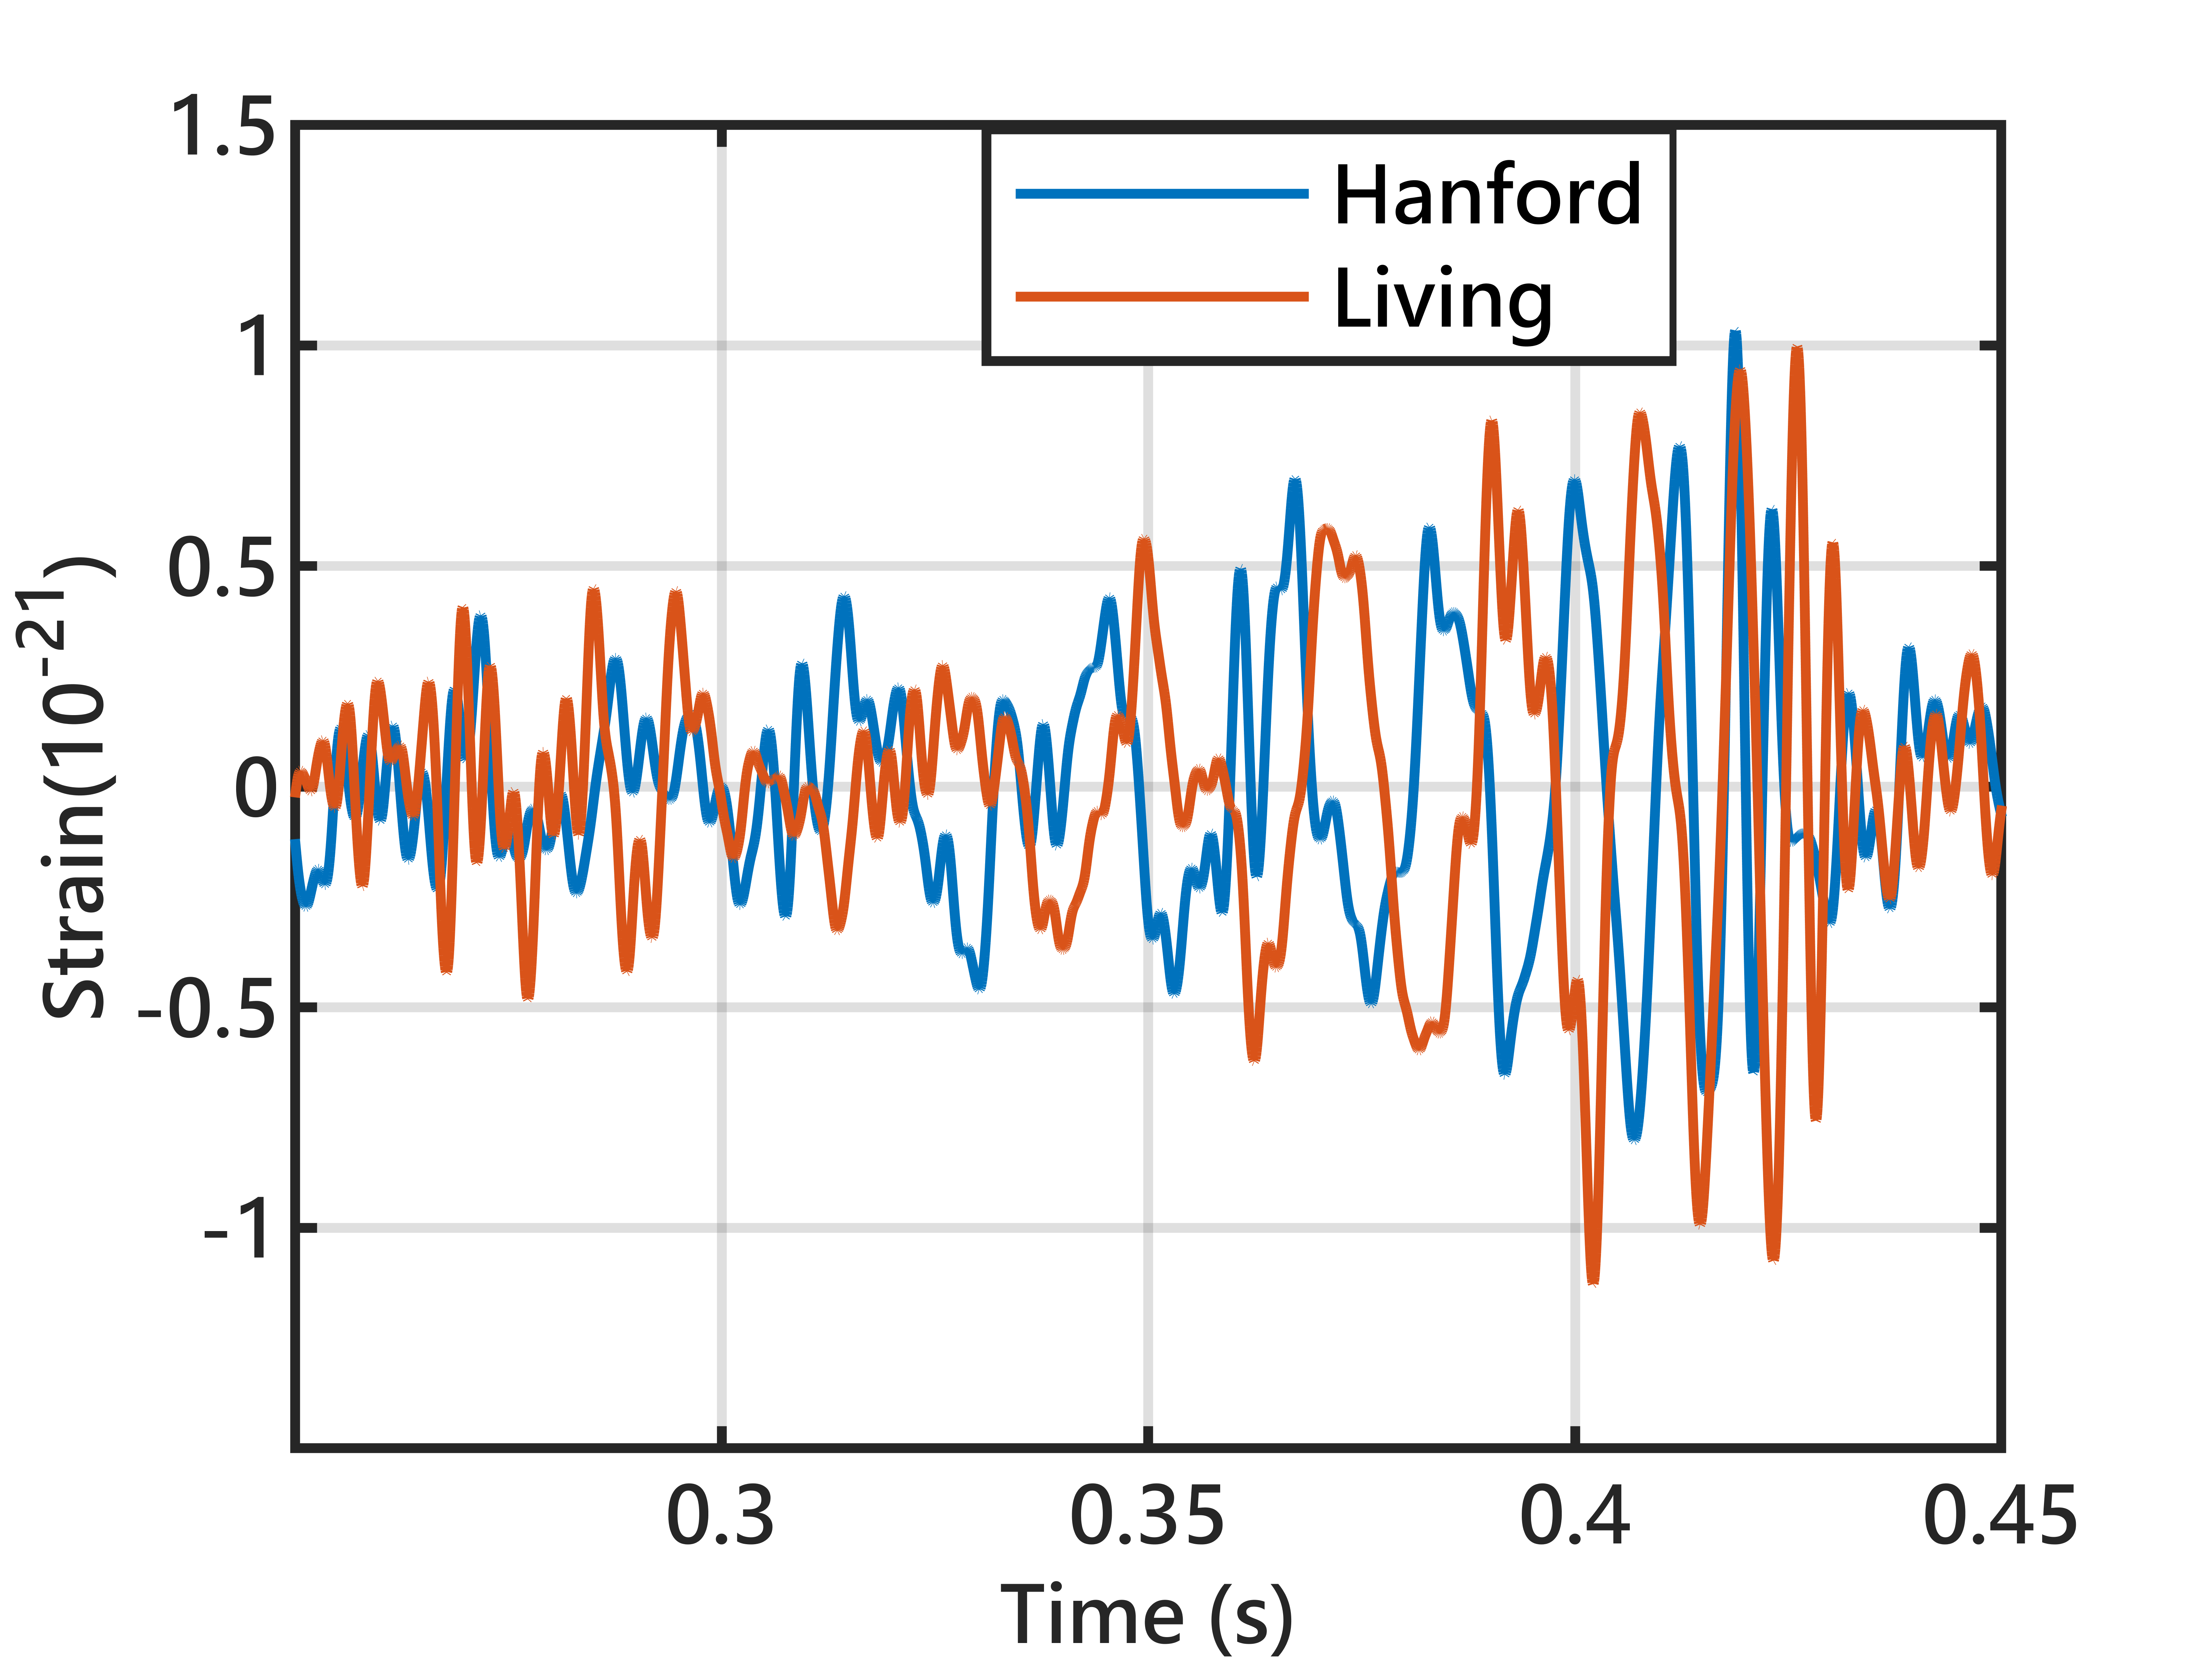
\includegraphics[width = 0.45\hsize]{未修正的引力波数据.png}}
	\subfigure[修正后的引力波波形]{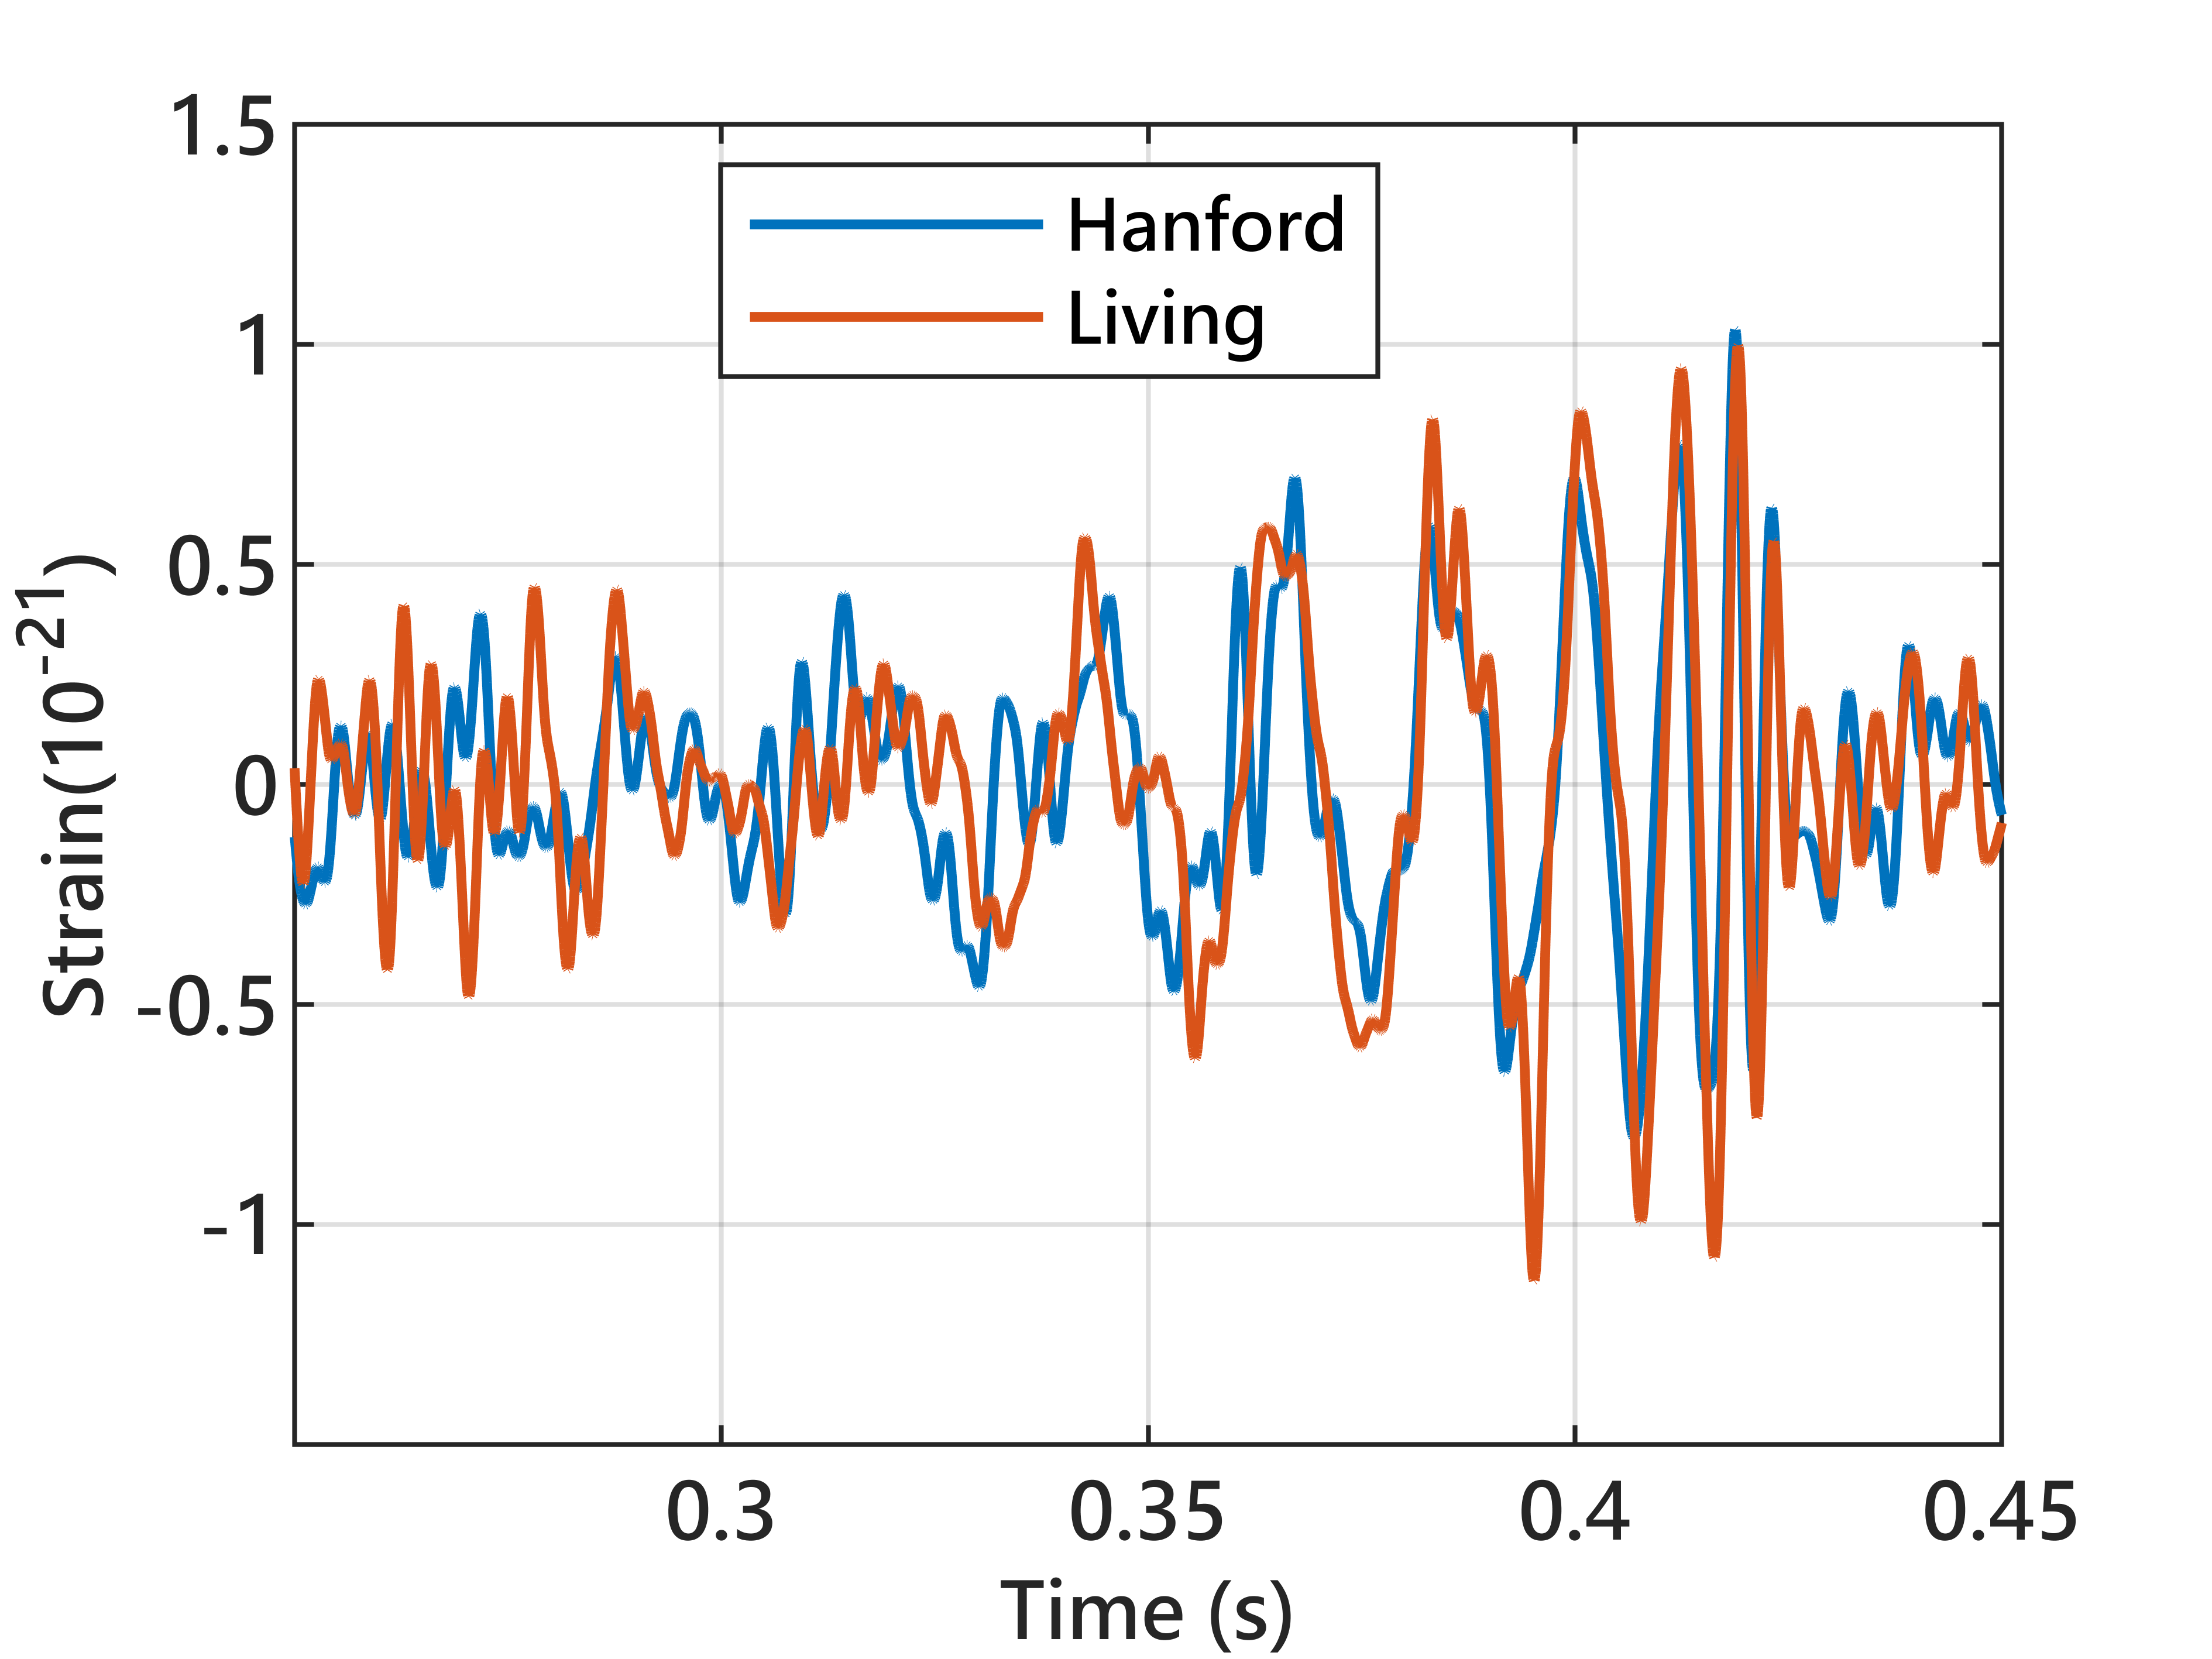
\includegraphics[width = 0.45\hsize]{引力波.png}}
	\caption{引力波波形}
\end{figure}

LIGO Hanford和Livingston探测器在UTC时间为2015年9月14日9:50:45左右探测到了编号为GW150914的引力波。为了更值地看到引力波波形,原始数据经过30Hz-350Hz的滤波器,因为这是探测器灵敏度最高的频率带。同时应用带阻滤波器消除仪器产生的高频谱噪声。经过处理后得到图1(a)的图像。 这时Living和Hanford的波形还存在较大差异, 因为Living和Hanford的地理位置不同,Living首先探测到引力波信号,比Hanford早6.9ms,而且两者的探测方向相反。 所以图1(a)的数据需要修正。 修正后的引力波波形如图1(b)所示。

\begin{figure}[!htbp]
	\centering
	\subfigure[Hanford 的时频图]{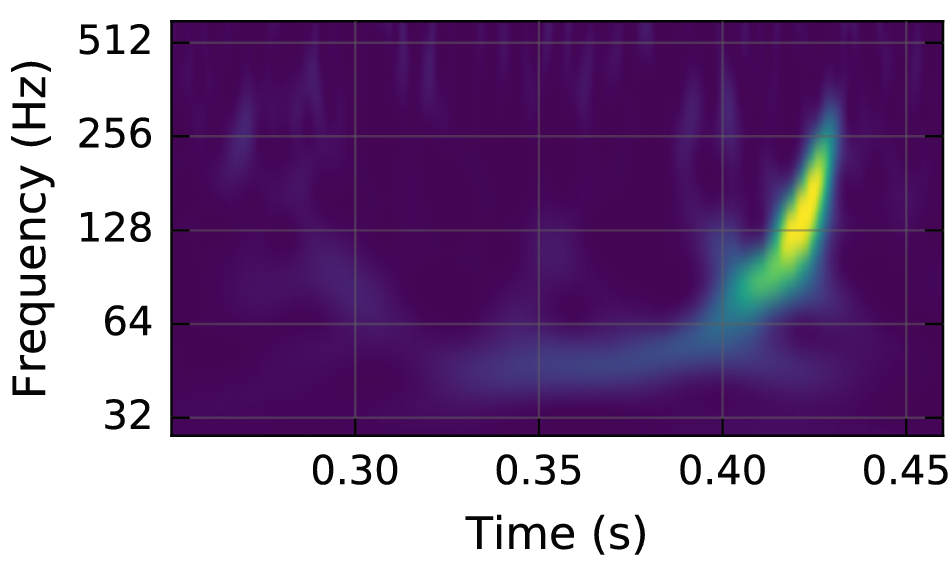
\includegraphics[width = 0.45\hsize]{fig1-freqtime-H.png}}
	\subfigure[Living 的时频图]{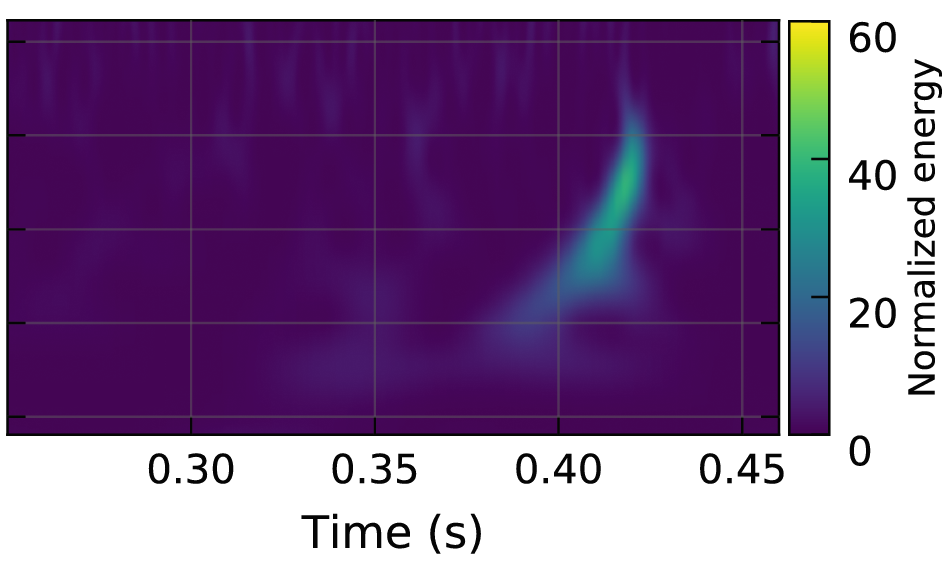
\includegraphics[width = 0.45\hsize]{fig1-freqtime-L.png}}
	\caption{时频图}
\end{figure}
图2表示Hanf和Living的引力波能量随时间和频率变化的图像。从图中可以看出,随着时间和频率的增大,引力波能量也在增大。从0.3s开始,引力波周期减小,所以频率开始增大。在0.42s左右,能量迅速下降,频率趋于稳定。最后,引力波的瞬时频率高于200Hz。整个过程持续了大概0.15s。

广义相对论中,质量在加速的情况下会产生引力波。由于波形表现出了至少八个振荡周期,所以存在一个或多个质量在振荡。引力波频率和能量的增大也表示在这段时间里引力波源的振荡频率也在增大。在引力波频率和能量都在增大时,天体的轨道运动只有一个合理的解释:引力波向外辐射能量,它产生了天体运动唯一的阻力,使得两个天体在不断靠近,频率不断增大且放大了引力波辐射的能量。

我们将证明,随观测到的频率演化唯一合理的解释是,该系统由两个黑洞组成,它们相互环绕,绕后合并在一起。

\textbf{确定能量最大时对应的频率}$f_{\rm GW}|_{\rm max}$ : 在证明时,一个非常重要的物理量是能量最大时的频率值。 利用图1的峰值或者图2的最亮点附近的过零点,我们保守地计算处该值
\begin{equation}
f_{\rm GW}|_{\rm max} \sim 150{\rm Hz},
\end{equation}
因此我们可以把引力波源的轨道运动解释为,天体做轨道运动时,轨道角频率不超过某个值
\begin{equation}
\omega_{\rm Kep}|_{\rm max}=\frac{2\pi f_{\rm GW}|_{\rm max}}{2} = 2\pi \times 75 {\rm Hz}
\end{equation}

\textbf{确定引力波源的质量量级}:爱因斯坦发现无迹质量四极矩为$Q_{ij}$的系统在视界距离为$d_L$产生的引力波形变$h$为
\begin{equation}
h_{ij}=\frac{2G}{c^4d_L}\frac{{\rm d^2}Q_{ij}}{{\rm d}t^2}
\end{equation}
引力波辐射能量的速率可以由四极质量公式推出
\begin{equation}
\label{E4}
\begin{aligned} \frac{\mathrm{d} E_{\mathrm{GW}}}{\mathrm{d} t}=& \frac{c^{3}}{16 \pi G} \iint|\dot{h}|^{2} \mathrm{d} S=\frac{1}{5} \frac{G}{c^{5}} \sum_{i, j=1}^{3} \frac{\mathrm{d}^{3} Q_{i j}}{\mathrm{d} t^{3}} \frac{\mathrm{d}^{3} Q_{i j}}{\mathrm{d} t^{3}} \\ & \text { where }|\dot{h}|^{2}=\sum_{i, j=1}^{3} \frac{\mathrm{d} h_{i j}}{\mathrm{d} t} \frac{\mathrm{d} h_{i j}}{\mathrm{d} t} \end{aligned}
\end{equation}
其积分区域为半径为$d_L$的球。方程(\ref{E4})表示当轨道天体的速度远小于光速且引力波形变也不大时的轨道能量损失速率。在频率达到$f_{\rm GW}|_{\rm max}$前,我们会一直使用它。

对于一个双天体系统,我们使用$m_1, m_2$表示两天体的质量,使用$M=m_1+m_2$表示天体的总质量,$\mu = m_1m_2/M$表示减少的质量,质量系数为$q=m_1/m_2$,假设$m_1\geq m_2$即$q\geq 1$.我们可以定义chirp mass 为$\mathscr{M}$来表示双天体引力波源系统向外辐射引力波的表达式
\begin{equation}
\mathscr{M} = \frac{(m_1m_2)^{3/5}}{(m_1+m_2)^{1/5}}
\end{equation}

使用牛顿运动定律,万有引力定律和爱因斯坦的引力波光度四极方程,导出了一个简单的公式,把引力波的频率与频率导数和chirp mass联系起来。
\begin{equation}
\label{E6}
\mathscr{M}=\frac{c^{3}}{G}\left(\left(\frac{5}{96}\right)^{3} \pi^{-8}\left(f_{\mathrm{GW}}\right)^{-11}\left(\dot{f}_{\mathrm{CW}}\right)^{3}\right)^{1 / 5}
\end{equation}
只要牛顿运动定律有效,这个公式就有效。

所以我们可以通过观测数据使用引力波的频率和频率导数计算任意时刻的chirp mass。当然,$\mathscr{M}$的确切值是多少并不重要,为了简单起见,我们设$\mathscr{M}=30M_\odot$。

chirp mass在$f_{\rm GW}|_{\rm max}<150{\rm Hz}$会保持不变,这样就给解释轨道运动提供了有力的支持。引力波应变的能量随频率增加也支持这样的解释,且计算中这些公式的假设是适用的:1. 双星系统的速度远小于光速;2. 轨道运动的半径在不断减少;3. 使用开普勒定律来描述周期。

chirp mass 还可以换一种计算方法
\begin{equation}
f_{\mathrm{GW}}^{-8 / 3}(t)=\frac{(8 \pi)^{8 / 3}}{5}\left(\frac{G \mathscr{M}}{c^{3}}\right)^{5 / 3}\left(t_{c}-t\right)
\end{equation}
这个方程不包含频率的导数,所以可以直接通过应变数据的过零点的时间间隔来计算$\mathscr{M}$.常数$t_c$是合并时刻。图3更直观的展示了这个现象。

\section{证明天体是致密的}

\end{document}